\documentclass[a4paper]{article}
\usepackage[spanish,es-tabla]{babel}	% trabajar en español
\spanishsignitems	
%\usepackage{simplemargins}

%\usepackage[square]{natbib}
\usepackage{amsmath}
\usepackage{amsfonts}
\usepackage{amssymb}
\usepackage{bbold}
\usepackage{graphicx}
\usepackage{blindtext}
\usepackage{hyperref}
\usepackage{amsthm}
\newtheorem{theorem}{Teorema}
\newtheorem{lemma}{Lema}
\usepackage{algorithm}
%\usepackage{algorithmic}
\usepackage{algpseudocode}
%\usepackage{algorithm2e}
\usepackage{booktabs}
\usepackage[export]{adjustbox}
\setcounter{MaxMatrixCols}{20}
\begin{document}
\pagenumbering{arabic}

\Large
 \begin{center}
\textbf{Simulación MC Modelo de Ising}\


\hspace{10pt}

% Author names and affiliations
\large
%Lic. Julio A. Medina$^1$ \\
Julio A. Medina \\
\hspace{10pt}
\small  
 Universidad de San Carlos\\
Escuela de Ciencias Físicas y Matemáticas\\
Maestría en Física\\
\href{mailto:julioantonio.medina@gmail.com}{julioantonio.medina@gmail.com}\\

\end{center}

\hspace{10pt}

\begin{abstract}
En mecánica estadística el Modelo de Ising para la modelación teórica de un material ferromagnético consiste en considerar las interacciones de corto rango del momento dipolar magnético de spins moleculares. Los spins se configuran en un retículo n-dimensional y están discretizados. 

\end{abstract}

\normalsize
\section{Introducción}
\subsection{Modelo de Ising}
El modelo de Ising considera las interacciones ferromagnéticas entre las moléculas de un material como un modelo discreto, esto consiste en asignar un valor discreto a la orientación relativa del momento dipolar magnético(spin), se asigna $+1$ a una orientación paralela al eje $y$ en el retículo formado por las posiciones discretizadas de las moléculas. ver fig. 1. y se le asigna $-1$ a la orientación anti-paralela. 

\begin{figure}[H]
\begin{center}
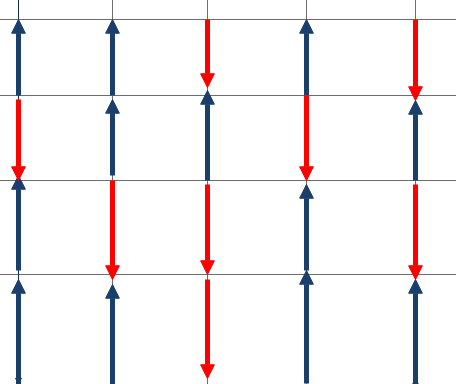
\includegraphics[scale=0.4]{LatticeIsing.png} 
\end{center} 
\caption{Retículo de spins}
\end{figure}

Se considera en el análisis la interacción entre spines vecinos $\sigma_{i}$, donde $\sigma_i=\pm1$ representa el spin en la  posición $(x,y)$ del retículo, la fuerza de la interacción entre vecinos se rige por una constante $J$ de modo que el Hamiltoniano del sistema se puede escribir de la siguiente manera.
\begin{equation}
\label{H1}
\mathcal{H}=-J\sum_{\langle i j\rangle}\sigma_i \sigma_j-H\sum_{i=1}^{N}\sigma_i
\end{equation}
donde $H$ es un campo magnético externo aplicado a la región donde se encuentra el retículo de moléculas ,$N$ es el numero total de moléculas en el retículo y la energía $J$ se puede interpretar como un parámetro cuántico de interacción electrostática, en la primera sumatoria se hace la observación que $\langle i j\rangle$ significa la suma de las interacciones de los vecinos más cercanos(vecinos próximos), estos son por ejemplo si se toma a la posición $(x,y)$ sus vecinos serian ${(x,y+1),(x,y-1),(x-1,y),(x+1,y)}$, los vecinos se pueden ver en color azul en la fig 2. y la posición $(x,y)$ se aprecia en color rojo. El primer termino de \ref{H1} representa la energías de interacción introducidas para llevar a un estado ferromagnético ordenado, el segundo termino representa la interacción entre el campo magnético aplicado $H$ y los spines del sistema está interacción es de carácter puramente paramagnético.
\begin{figure}[H]
\begin{center}
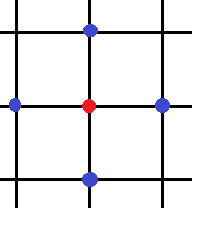
\includegraphics[scale=0.4]{Neighbor.png} 
\end{center} 
\caption{Vecinos mas cercanos}
\end{figure}
Tomando el caso en le que $H=0$ la ecuación \ref{H1} se convierte en 
\begin{equation}
\label{H2}
\mathcal{H}=-J\sum_{(i\sim j)}\sigma_i \sigma_j
\end{equation}
Para resolver el problema de Ising se tiene que encontrar la función de partición canónica
\begin{equation}\label{partition}
Z(T,H,N)=\sum_{\{ \sigma_i\}}\exp(-\beta \mathcal{H})
\end{equation}
con $\beta=\frac{1}{K_B T}$, $K_B$ es la constante de Boltzman, y $T$ es la temperatura en Kelvins.\\
\section{Metodología}
\subsection{Método de Monte Carlo}
\subsubsection{Ecuación maestra}
Se introduce lo que se conoce como ecuación maestra(ver \cite{silvio}) para la evolución temporal de procesos estocásticos Markovianos. Si $P(x,t)$ es la probabilidad de encontrar un sistema en el estado microscópico $y$, en el tiempo $t$. Derivando esta probabilidad se tiene
\begin{equation}
\frac{\partial}{\partial t}P(y,t)=T_0-T_f
\end{equation}
donde la tasa de probabilidad de cambiar al estado $y$ esta dada por
\begin{equation}
T_0=\sum_{y'}P(y',t)w(y'\rightarrow y)
\end{equation}
donde $w(y'\rightarrow y)$ puede ser interpretado como la probabilidad que el sistema pase del estado $y'$ al estado $y$ en un intervalo de tiempo muy pequeño. Análogamente la tasa de probabilidad de cambio $y\rightarrow y'$ esta dada por
\begin{equation}
T_f=P(y,t)\sum_{y'}w(y\rightarrow y')
\end{equation}
La ecuación maestra se convierte en 
\begin{equation}\label{masterEq}
\frac{\partial}{\partial t}P(y,t)=\sum_{y'}\Big[P(y',t)w(y'\rightarrow y)-P(y,t)w(y\rightarrow y')\Big]
\end{equation}
Para un estado estacionario $P(y,t)$ no es una función explicita del tiempo, por lo que para el equilibrio se tiene
\begin{equation}
\frac{\partial}{\partial t}P(y,t)=0
\end{equation}
Entonces se tiene la siguiente condición de equilibrio llamado principio de balance detallado
\begin{equation}\label{equi}
P(y',t)w(y'\rightarrow y)=P(y,t)w(y\rightarrow y')
\end{equation}
\subsection{Metodo de Monte Carlo}
El estudio de sistemas en equilibrio en mecánica estadística  esta interesado en el calculo de promedios de la forma
\begin{equation}\label{MCavg}
\langle A\rangle=\frac{\displaystyle \sum_{C} A(C) \exp(-\beta\mathcal{H})}{\displaystyle\sum_{C} \exp(-\beta\mathcal{H})}
\end{equation}
donde  la suma indica que se toman en cuenta todas las posibles configuraciones microscópicas del sistema asociado con el Hamiltoniano $\mathcal{H}$, para el caso del modelo de Ising 2D se tiene un retículo de $N=n\times n$ sitios, esto significa que la suma en \ref{MCavg} se hace sobre $2^N=2^{n^2}$ configuraciones. El hecho que el numero de configuraciones crece como $2^{n^2}$ hace que no sea practico utilizar este tipo de expresión para realizar cálculos numéricos. La solución consiste en realizar promedios sobre un numero mucho mas pequeño de las configuraciones de equilibrio mas representativas  del sistema,
\begin{equation}\label{MCavg2}
\langle A\rangle=\frac{1}{M}\sum^M_{i=1}A_i
\end{equation}
Es importante saber bajo que condiciones se puede realmente obtener el valor esperado de la cantidad $A$ de este promedio aritmético sobre las configuraciones representativas $M$, también es importante saber como seleccionar el numero $M$ de configuraciones representativas. \\
De acuerdo con el método de Monte Carlo se selecciona una secuencia de configuraciones independientes, estas se denominan cadenas de Markov. Algunas de las configuraciones iniciales están lejos del equilibrio pero como función del tiempo se generan muchas mas configuraciones de equilibrio que son utilizadas para promediar \ref{MCavg2}.\\
Como ya fue discutido si se identifica a $w(y\rightarrow y')$ como la probabilidad de transición por unidad de tiempo del estado $y$ a $y'$ se tiene a la ecuación maestra \ref{masterEq} y la condición \ref{equi}.\\
En equilibrio, esto es después de tomar en cuenta varios términos de la secuencia las probabilidades deberían tender a los valores de Gibbs,
\begin{equation}
P_0(y)=\frac{1}{Z}\exp[-\beta\mathcal{H}(y)]
\end{equation}
donde $Z$ la función de partición canónica esta definida en \ref{partition}. De la condición \ref{equi} se tiene
\begin{equation}
P_0(y)w(y\rightarrow y')=P_0(y')w(y'\rightarrow y)
\end{equation}.
Se escogen probabilidades  que satisfacen 
\begin{equation}\label{probTans1}
\frac{w(y\rightarrow y')}{w(y'\rightarrow y)}=\exp (-\beta \Delta \mathcal{H})
\end{equation}
donde $\Delta\mathcal{H}=\mathcal{H}(y')-\mathcal{H}(y)$ es la diferencia de energías entre las configuraciones $y$ y $y'$.\\
Otras dos probabilidades de transición utilizadas en el las simulaciones de monte Carlo son el algoritmo de Glauber y la prescripción de Metrópolis, en esta simulación se ha escogido a la prescripción de Metrópolis,
\begin{equation}
w(y\rightarrow y')=\left\{
        \begin{array}{ll}
            \frac{1}{\tau}\exp (-\beta \Delta \mathcal{H}), & \quad\;\,\,\,\, \Delta\mathcal{H}> 0 \\\\
            \frac{1}{\tau}, & \quad\quad \Delta\mathcal{H}< 0
        \end{array}
    \right.
\end{equation}
donde el tiempo $\tau$ se interpreta como "step de Monde Carlo", se ha escogido $\tau=1$.

\subsubsection{Método de Monte Carlo para el Modelo de Ising}
Se presentan a continuación los pasos del método de Monte Carlo y el diagrama de flujo para generar la cadena de Markov.
\begin{enumerate}
\item Escoger una configuración inicial de spins en el retículo.
\item Se selecciona un sitio al azar y se calcula la energía en ese sitio para las interacciones con los vecinos mas cercanos. 
\item Verificar el signo de $E$.
\item Si $E$ es positiva se hace el cambio de spin en el sitio indicado, esto es $\sigma_i=-\sigma_i$.
\item Si $E$ es negativa pero $\exp(-\beta \Delta \mathcal{H})>p_t$, donde $p_t$ es un numero aleatorio entre $0$ y $1$, se cambia al spin, de otra manera se reinicia el ciclo.
\end{enumerate}
es fácil ver que estos pasos reproducen la prescripción de Metrópolis.
\pagebreak
\begin{figure}[H]
\begin{center}
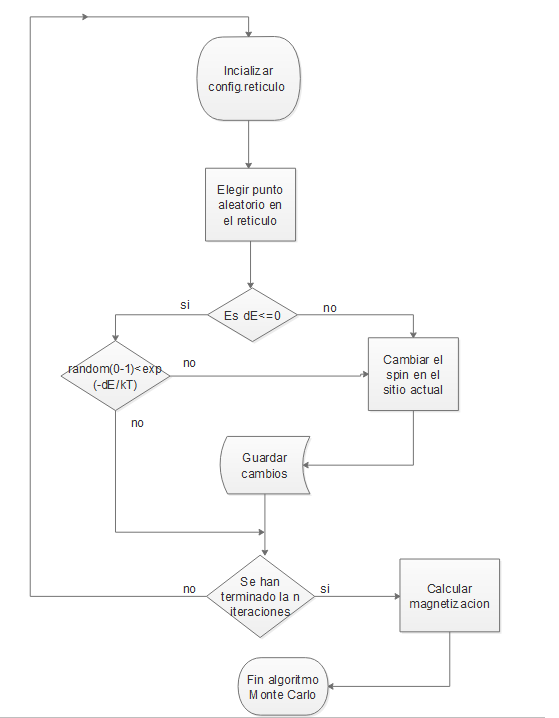
\includegraphics[scale=0.9]{FluxDiagram.png} 
\end{center} 
\caption{Diagrama de flujo}
\end{figure}
\begin{thebibliography}{99}
%% La bibliografía se ordena en orden alfabético respecto al apellido del 
%% autor o autor principal
%% cada entrada tiene su formatado dependiendo si es libro, artículo,
%% tesis, contenido en la web, etc
%Las fuentes de consulta se citan en forma organizada y homogénea, tanto de los libros, de los artículos y, en general, de las obras consultadas, que fueron indispensables indicar o referir en el contenido del trabajo.

\bibitem{silvio}Silvio R.A Salinas. \textit{Introduction to Statistical Physics}. Springer. First Edition.

\bibitem{}R.J. Baxter \textit{Exactly solved models in statistical physics}.Academic Press. First Edition. 

\bibitem{}R.K. Pathria \textit{Statistical Mechanics}. Elsevier.Third Edition.
%¨\bibitem{}\textit{Finite Difference method}.\url{https://en.wikipedia.org/wiki/Finite_difference_method}

%\bibitem{Feynman} 
%\bibitem{Hopfield} J.J. Hopfield. \textit{Neural Networks and physical systems with emergent collective computational abilities}. \url{https://doi.org/10.1073/pnas.79.8.2554}


%\bibitem{McCulloch} Warren S. McChulloch, Walter H. Pitts. \textit{A LOGICAL CALCULUS OF THE IDEAS IMMANENT IN NERVOUS ACTIVITY}. \url{http://www.cse.chalmers.se/~coquand/AUTOMATA/mcp.pdf}



\end{thebibliography}
\end{document}

